%%%%%%%%%%%%%%%%%%%%%%%%%%%%%%%%%%%%%%%%%
% Beamer Presentation
% LaTeX Template
% Version 1.0 (10/11/12)
%
% This template has been downloaded from:
% http://www.LaTeXTemplates.com
%
% License:
% CC BY-NC-SA 3.0 (http://creativecommons.org/licenses/by-nc-sa/3.0/)
%
%%%%%%%%%%%%%%%%%%%%%%%%%%%%%%%%%%%%%%%%%

%----------------------------------------------------------------------------------------
%	PACKAGES AND THEMES
%----------------------------------------------------------------------------------------

%\pdfminorversion=4
\documentclass[10pt]{beamer}

\mode<presentation> {

% The Beamer class comes with a number of default slide themes
% which change the colors and layouts of slides. Below this is a list
% of all the themes, uncomment each in turn to see what they look like.

%\usetheme{default}
%\usetheme{AnnArbor}
%\usetheme{Antibes}
%\usetheme{Bergen}
%\usetheme{Berkeley}
%\usetheme{Berlin}
%\usetheme{Boadilla}
%\usetheme{CambridgeUS}
%\usetheme{Copenhagen}
%\usetheme{Darmstadt}
%\usetheme{Dresden}
%\usetheme{Frankfurt}
%\usetheme{Goettingen}
%\usetheme{Hannover}
%\usetheme{Ilmenau}
%\usetheme{JuanLesPins}
%\usetheme{Luebeck}
%\usetheme{Madrid}
%\usetheme{Malmoe}
%\usetheme{Marburg}
%\usetheme{Montpellier}
%\usetheme{PaloAlto}
%\usetheme{Pittsburgh}
%\usetheme{Rochester}
%\usetheme{Singapore}
%\usetheme{Szeged}
%\usetheme{Warsaw}


\usetheme[sectionpage=none]{metropolis} % https://github.com/matze/mtheme

% As well as themes, the Beamer class has a number of color themes
% for any slide theme. Uncomment each of these in turn to see how it
% changes the colors of your current slide theme.

%\usecolortheme{albatross}
%\usecolortheme{beaver}
%\usecolortheme{beetle}
%\usecolortheme{crane}
%\usecolortheme{dolphin}
%\usecolortheme{dove}
%\usecolortheme{fly}
%\usecolortheme{lily}
%\usecolortheme{orchid}
%\usecolortheme{rose}
%\usecolortheme{seagull}
%\usecolortheme{seahorse}
%\usecolortheme{whale}
%\usecolortheme{wolverine}

%\setbeamertemplate{footline} % To remove the footer line in all slides uncomment this line
%\setbeamertemplate{footline}[page number] % To replace the footer line in all slides with a simple slide count uncomment this line

%\setbeamertemplate{navigation symbols}{} % To remove the navigation symbols from the bottom of all slides uncomment this line
}


\usefonttheme{professionalfonts}
 % required for mathspec
\usepackage{mathspec}
%\setsansfont[BoldFont={Fira Sans},Numbers={OldStyle}]{Fira Sans Light}
\setsansfont[BoldFont={Fira Sans}]{Fira Sans Light}
\setmathsfont(Digits)[Numbers={Lining,Proportional}]{Fira Sans Light}



\usepackage{graphicx} % Allows including images
\usepackage{booktabs} % Allows the use of \toprule, \midrule and \bottomrule in tables
\usepackage{tikz}
\usepackage{tikz-3dplot}
\usepackage{tikz-dimline}
\usetikzlibrary{arrows.meta}
\usetikzlibrary{calc,angles,quotes} % angles, quotes = http://www.texample.net/tikz/examples/angles-quotes/
\usetikzlibrary{plotmarks} % https://tex.stackexchange.com/questions/140963/draw-a-filled-circle-at-every-point-of-a-tikz-plot#140967
%\usepackage{textpos}
\usepackage{pgf}

\usepackage{etoolbox} % For ifdef in footer
\usepackage[absolute, overlay]{textpos}

\usepackage{environ}
%%%%%%%%%%%%%%%%%%
% Code to scale a tikzpicture to textwidth (keeping correct font dimension).
% Preso da https://tex.stackexchange.com/questions/6388/how-to-scale-a-tikzpicture-to-textwidth#6391
% Necessita di \usepackage{environ} nel preambolo
% Usato cosi'
% \begin{scaletikzpicturetowidth}{\textwidth}
%   \begin{tikzpicture}[scale=\tikzscale]
%     \draw...
%   \end{tikzpicture}
% \end{scaletikzpicturetowidth}
%
\makeatletter
\newsavebox{\measure@tikzpicture}
\NewEnviron{scaletikzpicturetowidth}[1]{%
  \def\tikz@width{#1}%
  \def\tikzscale{1}\begin{lrbox}{\measure@tikzpicture}%
  \BODY
  \end{lrbox}%
  \pgfmathparse{#1/\wd\measure@tikzpicture}%
  \edef\tikzscale{\pgfmathresult}%
  \BODY
}
\makeatother














\DeclareGraphicsExtensions{.pdf, .png, .jpg} % Se due immagini hanno lo stesso nome sceglile secondo l'ordine di filetype qui
\graphicspath{ {./img/} }					 % Path delle immagini 





\newcommand{\nologo}{\setbeamertemplate{logo}{}}

% TODO use real file not test_
% FILE GENERATED AUTOMATICALLY

\newcommand{\myname}{Francesco Forcher}
\newcommand{\crystalname}{TCP76}
\newcommand{\runnumber}{5870}
\newcommand{\rundate}{2017-12-04}
\newcommand{\particletype}{Xenon}
\newcommand{\particleenergy}{95.6 GeV}

\newcommand{\xmin}{-0.875}
\newcommand{\xmax}{0.525}
\newcommand{\ymin}{-0.875}
\newcommand{\ymax}{0.525}

\newcommand{\torsionm}{1.8}
\newcommand{\torsionq}{-14.7}
\newcommand{\torsionmerr}{0.5}
\newcommand{\torsionqerr}{0.6}


%----------------------------------------------------------------------------------------
%	TITLE PAGE
%----------------------------------------------------------------------------------------

\title[Analysis of high statistics channeling run \runnumber, crystal \crystalname]
{Analysis of high statistics run \runnumber of the crystal \crystalname in the channeling position, to determine the bending angle and efficiency for different
angular cuts.} % The short title appears at the bottom of every slide, the full title is only on the title page
\subtitle{Laurea triennale in Fisica}


% \author{Francesco Forcher} % Your name
% \institute[UNIPD] % Your institution as it will appear on the bottom of every slide, may be shorthand to save space
% {
% Supervisors: \\ % Your institution for the title page
% M. Zanetti (UNIPD) \\
% D. Mirarchi (UNIPD) \\
% S. Redaelli (UNIPD) \\
% %\medskip
% %\textit{francesco.forcher@cern.ch} % Your email address
% }
%\author{Francesco Forcher} % Your name
\institute[UNIPD] % Your institution as it will appear on the bottom of every slide, may be shorthand to save space
{ }
\date{%
\today \\
\textit{Run date: 2017.05.16}\\
}%\vspace{\stretch{1}}} % Date, can be changed to a custom date

\logo{\begin{tikzpicture}[remember picture,overlay]%
\node[anchor=south west,yshift=1cm, xshift=0.95cm] at (current page.south west) {
\includegraphics[height=1cm]{img/CERN_LogoBadge.pdf}};
%\node[anchor=south west,yshift=1cm, xshift=2.5cm] at (current page.south west) {\includegraphics[height=1cm]{img/logoesigillo_unipd.pdf}};
%\node[anchor=east,yshift=-0.91cm, xshift=-1cm] at (current page.east) {\includegraphics[height=1.3cm]{img/logoesigillo_unipd.pdf}};
\node[anchor=south east,yshift=1cm, xshift=-0.85cm] at (current page.south east) {
\includegraphics[height=1cm]{img/be_dep_logo.pdf}};
\end{tikzpicture}}
% \logo{\begin{tikzpicture}[remember picture,overlay]%
% \node[anchor=south west,yshift=1cm, xshift=0.95cm] at (current page.south west) {\includegraphics[height=1cm]{img/logoesigillo_unipd.pdf}};
% \node[anchor=south west,yshift=1cm, xshift=4.5cm] at (current page.south west) {
\includegraphics[height=1cm]{img/CERN_LogoBadge.pdf}};
% %\node[anchor=east,yshift=-0.91cm, xshift=-1cm] at (current page.east) {\includegraphics[height=1.3cm]{img/logoesigillo_unipd.pdf}};
% \node[anchor=south east,yshift=1cm, xshift=-0.85cm] at (current page.south east) {
\includegraphics[height=1cm]{img/be_dep_logo.pdf}};
% \end{tikzpicture}}

\begin{document}


\addtobeamertemplate{frametitle}{}{%
\begin{tikzpicture}[remember picture,overlay]
\node[anchor=north east,yshift=5pt, xshift=5pt] at (current page.north east) {
\includegraphics[height=1cm]{img/CERN_LogoBadge_no_transparency.pdf}};
\end{tikzpicture}}




\begin{frame}
\titlepage % Print the title page as the first slide
\end{frame}

\nologo

% \begin{frame}
% \frametitle{Overview} % Table of contents slide, comment this block out to remove it
% \tableofcontents % Throughout your presentation, if you choose to use \section{} and \subsection{} commands, these will automatically be printed on this slide as an overview of your presentation
% \end{frame}

%----------------------------------------------------------------------------------------
%	PRESENTATION SLIDES
%----------------------------------------------------------------------------------------

\setbeamertemplate{frame footer}{\insertsection}
\metroset{titleformat section=smallcaps}
\metroset{titleformat frame=smallcaps}

% %------------------------------------------------
% \section{Introduzione}
% %------------------------------------------------
% 
% \begin{frame}
% \frametitle{Introduzione}
% Quando un fascio di particelle ad alta energia impatta su un materiale cristallino,
% possono avvenire entro uno specifico range angolare dei fenomeni di interazioni coerenti,
% con risultati differenti dal tradizionale scattering amorfo.
% 
% In particolare, curvando i cristalli, essi aquisiscono la proprietà di deviare le particelle secondo degli
% angoli ben definiti, aprendo la possibilità a precise manipolazioni del fascio.
% Tali fenomeni possono essere dunque sfruttati per la collimazione 
% del fascio negli acceleratori di particelle,
% come viene investigato all'esperimento \alert{\textbf{UA9}} del CERN.
% 
% In questa tesi, verranno analizzati i dati di questo esperimento per migliorare la routine
% di simulazione \textit{SixTrack}, utilizzata negli studi di collimazione.
% \end{frame}

%------------------------------------------------
\section{Introduzione}
%------------------------------------------------

\begin{frame}
\frametitle{Introduzione}
\begin{columns}[c] % The "c" option specifies centered vertical alignment while the "t" option is used for top vertical alignment

\column{.55\textwidth} % Left column and width
\vspace*{-0.3cm}%
\begin{block}{}
\begin{itemize}
\item Quando un fascio di particelle impatta su un cristallo,
possono avvenire dei fenomeni di interazioni coerenti.

\item Curvando i cristalli, essi possono deviare le particelle secondo
angoli ben definiti.
\end{itemize}
\end{block}

\column{.45\textwidth} % Right column and width
\begin{figure}
\includegraphics[width=0.6\linewidth]{foto_cristallo}
\caption{ \footnotesize \itshape
Un cristallo nel suo holder.
}
\end{figure}
\end{columns}
\vspace*{-0.9cm}
\begin{columns}[c]
% Quando un fascio di particelle impatta su un cristallo,
% possono avvenire dei fenomeni di interazioni coerenti, differenti dal tradizionale scattering amorfo.
% 
% In particolare, curvando i cristalli, essi aquisiscono la proprietà di deviare le particelle secondo degli
% angoli ben definiti, aprendo la possibilità a precise manipolazioni del fascio.
\column{\textwidth}
\begin{block}{}
\begin{itemize}
\item L'esperimento \alert{\textbf{UA9}} investiga come tali fenomeni possono essere sfruttati per la collimazione negli
acceleratori di particelle.

\item In questa tesi verranno analizzati i dati di UA9 per migliorare
\textit{SixTrack}, routine utilizzata negli studi di collimazione.
\end{itemize}
\end{block}

\column{0cm}

\end{columns}
\end{frame}

%------------------------------------------------
\subsection{I cristalli per la collimazione}
% 
% \begin{frame}
% \frametitle{Introduzione}
% \begin{columns}[c] % The "c" option specifies centered vertical alignment while the "t" option is used for top vertical alignment
% 
% \column{.55\textwidth} % Left column and width
% \vspace*{-0.8cm}%
% \begin{block}{Materiale}
% I cristalli sono fatti in silicio, a causa dell'elevato
% grado di purezza raggiungibile oggi grazie all'industria dei semiconduttori.
% Un holder in metallo poi esercita delle forze per curvarli. Possono dividersi in STF o QMP 
% a seconda del metodo di fabbricazione e curvatura.
% \end{block}
% 
% \begin{block}{Setup}
% I cristalli in questa tesi sono stati testati sulla linea di estrazione H8, nella North Area del CERN.
% \end{block}
% 
% \column{.45\textwidth} % Right column and width
% \begin{figure}
% \begin{scaletikzpicturetowidth}{0.8\textwidth} % Vedi stili_float
% \input{img/diamond_cubic.tex}
% \end{scaletikzpicturetowidth}
% \caption{ \footnotesize \itshape
% Struttura cristallina del silicio.
% }
% \end{figure}\vspace*{-0.8cm}%
% %
% \begin{figure}
% \includegraphics[width=0.6\linewidth]{foto_cristallo}
% \caption{ \footnotesize \itshape
% Un cristallo nel suo holder.
% }
% \end{figure}


\end{columns}
\end{frame}


%------------------------------------------------
\section{Teoria}
%------------------------------------------------


\begin{frame}
\frametitle{Channeling e Volume reflection}
\begin{columns}[c] % The "c" option specifies centered vertical alignment while the "t" option is used for top vertical alignment

\column{.5\textwidth} % Left column and width
\begin{figure}
    {\footnotesize \itshape Channeling\vspace*{0.5cm}}
%   \def\svgwidth{0.9\textwidth}
%   \input{img/channeling_thetab_LaTeX.pdf_tex}
\includegraphics[width=\linewidth]{channeling_thetab.pdf}
\end{figure}

\column{.5\textwidth} % Left column and width
\begin{figure}
    {\footnotesize \itshape Volume reflection\vspace*{0.5cm}}
    \def\svgwidth{0.9\textwidth} % TODO TODO TODO Capire errore pdf_tex
    \input{img/volume_reflection_LaTeX.pdf_tex}
\end{figure}
\end{columns}
\begin{center}
$\theta_b \approx 150\ \mu\textrm{rad}, \theta_c \approx 10\ \mu\textrm{rad}, R \approx 10 \textrm{m}$
\end{center}
\end{frame}


\begin{frame}
\frametitle{Collimazione multistage attuale}

\begin{figure}
\includegraphics[width=0.8\textwidth]{collimazione.jpg}
\caption{Collimazione multistage presente attualmente.}
\end{figure}

\end{frame}



% %------------------------------------------------
% 
% 
% \begin{frame}
% \frametitle{Volume reflection}
% \begin{columns}[c] % The "c" option specifies centered vertical alignment while the "t" option is used for top vertical alignment
% 
% \column{.5\textwidth} % Left column and width
% \begin{figure}
%     \def\svgwidth{0.9\textwidth} % TODO TODO TODO Capire errore pdf_tex
%     \input{img/volume_reflection_LaTeX.pdf_tex}
% \end{figure}
% 
% \column{.5\textwidth} % Right column and width 
% Le particelle che entrano con un angolo ${\theta_\textrm{in}} > \theta_c$
% ma minore di $\theta_b$ vengono riflesse %da un piano cristallino 
% con un $\Delta \theta$ all'incirca costante chiamato $\theta_\textrm{VR}$.
% Questo processo è denominato \alert{volume reflection}.
% \end{columns}
% \end{frame}


%------------------------------------------------
\section{Apparato strumentale} 
%------------------------------------------------

\begin{frame}
\frametitle{Apparato strumentale}
\begin{figure}
\includegraphics[width=\linewidth]{apparato_strumentale_orig.pdf}
\caption{L'apparato strumentale. Risoluzione lineare $\approx 7\ \mu\textrm{m}$, risoluzione teorica angolo d'ingresso $\approx 2.8\ \mu\textrm{rad}$.}
\end{figure}
% L'apparato strumentale è composto da cinque detector a microstrip con un'area ciascuno di 3.8x3.8 $\textrm{cm}^2$.
% Possono ricostruire dunque sia l'angolo e la posizione d'entrata e di uscita delle particelle.
% Il fascio, situato nella linea d'estrazione H8 dell'SPS al CERN, è composto da protoni a $400\ \textrm{GeV} / \textrm{c}$  
\end{frame}

%------------------------------------------------



%------------------------------------------------
\section{Simulazioni} 
%------------------------------------------------

\begin{frame}
\frametitle{Istogramma deflessioni angolari sperimentale}
\begin{figure}
\only<1>{\includegraphics[width=\linewidth]{STF45_exp.pdf}}
\only<2>{\includegraphics[width=\linewidth]{esempio_scanang_roottext.pdf}}
\only<3>{\includegraphics[width=\linewidth]{STF45_exp_circle.pdf}}
\caption{\footnotesize \itshape
Istogramma delle deflessioni a seconda dell'angolo d'ingresso.
\only<2>{Possiamo vedere cinque regioni distinte: 1)~Amorphous, 2)~Channeling, 3)~Dechanneling, 4)~Volume reflection, 5)~Volume capture.}
\only<3>{La regione d'interesse di questa tesi, la transizione da Volume Reflection ad amorfo.}
}
\end{figure}
\end{frame}

%------------------------------------------------

\begin{frame}
\frametitle{Istogramma deflessioni: vecchia simulazione}
\begin{figure}
\includegraphics[width=\linewidth]{STF45_sim_closer.pdf}
\caption{\footnotesize \itshape Le vecchie simulazioni non rappresentavano adeguatamente la transizione.}
\end{figure}%
\end{frame}


% %------------------------------------------------
% \section{Analisi dati} 
% %------------------------------------------------
% 
% \begin{frame}
% \frametitle{Analisi dati}
% \begin{columns}[t] % The "c" option specifies centered vertical alignment while the "t" option is used for top vertical alignment
% 
% \column{.5\textwidth} % Left column and width
% \begin{figure}
% \includegraphics[width=\textwidth]{grafico_slices.png}
% \end{figure}
% \begin{figure}
% \includegraphics[width=1\textwidth]{slices_examples.pdf}
% \end{figure}\vspace{1cm}
% 
% 
% \column{.5\textwidth} % Right column and width
% \\
% La regione di transizione \'e stata sezionata verticalmente, ottentendo cos\'i la distribuzione
% delle particelle per ogni $\theta_\textrm{in}$.
% 
% Questa distribuzione unidimensionale si presenta come una somma di due picchi gaussiani. La distribuzione \'e stata fittata attraverso
% l'uso della libreria di machine learning in python \alert{\texttt{scikit-learn}}, in particolare con un \texttt{gaussian mixture model}.
% Gli errori sono stati stimati con il metodo del bootstrap. 
% \end{columns}
% \end{frame}
% 
% %------------------------------------------------
% \section{Modello} 
% %------------------------------------------------
% 
% \begin{frame}
% \frametitle{Modello}
% \begin{columns}[c] % The "c" option specifies centered vertical alignment while the "t" option is used for top vertical alignment
% 
% \column{.5\textwidth} % Left column and width
% \begin{figure}
% \includegraphics[width=\textwidth]{ThModelSTF45.pdf}
% \end{figure}
% \begin{figure}
% \includegraphics[width=1\textwidth]{ThModelSTF45_means.pdf}
% \end{figure}
% 
% 
% \column{.5\textwidth} % Right column and width 
% Il modello \e' stato costruito sulla base dei parametri del cristallo, vale a dire $\theta_b$, $\theta_c$ e le sigma di scattering.
% 
% 
% \end{columns}
% \end{frame}

%------------------------------------------------
\section{Analisi dati e modellizazione} 
%------------------------------------------------

\begin{frame}
\frametitle{Analisi dati e modellizazione}
\begin{columns}[t] % The "c" option specifies centered vertical alignment while the "t" option is used for top vertical alignment

\column{.5\textwidth} % Left column and width
\vspace*{-1cm}
\begin{figure}
\caption{\footnotesize \itshape L'analisi}
\includegraphics[width=\textwidth]{grafico_slices.png}
\end{figure}\vspace{-0.8cm}
\begin{figure}
\includegraphics[width=\textwidth]{slices_examples.pdf}
\end{figure}\vspace{1cm}


\column{.5\textwidth} % Right column and width
\vspace*{-1cm}
\begin{figure}
\caption{ \footnotesize \itshape Il modello}
\includegraphics[width=\textwidth]{ThModelSTF45.pdf}
\end{figure}\vspace{-0.8cm}
\begin{figure}
\includegraphics[width=\textwidth]{ThModelSTF45_means.pdf}
\end{figure}

\end{columns}
\end{frame}

%------------------------------------------------
\section{Benchmarking delle simulazioni} 
%------------------------------------------------

\begin{frame}
\frametitle{Benchmarking delle simulazioni}
\begin{columns}[t] % The "c" option specifies centered vertical alignment while the "t" option is used for top vertical alignment

\column{.5\textwidth} % Right column and width
\vspace*{-1.7cm}
\begin{figure}
%\includegraphics[width=\textwidth]{bench_sigmas_STF99.pdf} STF45_sim_plus_smearing
\includegraphics[width=0.63\textwidth,angle=-90]{STF45_sim_plus_smearing.pdf}
\end{figure}\vspace{-0.8cm}
\begin{figure}
\includegraphics[width=\textwidth]{bench_weights_STF99.pdf}
\end{figure}



\column{.5\textwidth} % Left column and width
\vspace*{-0.8cm}

\begin{figure}
\includegraphics[width=\textwidth]{bench_means_STF99.pdf}
\end{figure}\vspace{-0.7cm}

\begin{figure}
\includegraphics[width=\textwidth]{rrossi_lossmap.pdf}\\
%{\vspace{-0.3cm}\tiny \itshape (Courtesy of R. Rossi)}
\end{figure}\vspace{1cm}


\end{columns}
\end{frame}

%------------------------------------------------
\section{Conclusioni} 
%------------------------------------------------

\begin{frame}
\frametitle{Conclusioni}

% \begin{itemize}
% \item I dati sperimentali dell'esperimento UA9 sono stati analizzati per creare un nuovo modello per la regione angolare di transizione
% tra i processi di volume reflection e scattering amorfo nei cristalli, da implementare nel software di simulazioni per la collimazione \texttt{SixTrack}.
% \item Le simulazioni sono state dunque analizzate per controllare che il nuovo modello riproducesse adeguatamente i dati sperimentali.
% \item Inoltre, altre simulazioni condotte su LHC con il nuovo modello sono risultate corrispondere meglio con i precedenti dati sperimentali, validando cos\'i il modello a differenti scale di energia.
% \item Sviluppi futuri potrebbero includere ulteriori benchmark in differenti condizioni di fascio, come altre scale di energia o altri tipi di particelle.
% \end{itemize}
\begin{itemize}
\item I dati di UA9 sono stati analizzati per creare un nuovo modello per la regione angolare di transizione
tra i processi di volume reflection e scattering amorfo nei cristalli, per il software \texttt{SixTrack}.
\item I dati simulati sono stati confrontati con i dati sperimentali, confermando il modello.
\item Altre simulazioni condotte su LHC sono risultate corrispondere meglio con i dati, validando il modello a differenti scale di energia.
\item Sviluppi futuri potrebbero includere ulteriori benchmark in differenti condizioni (altre scale di energia o tipi di particelle).
\end{itemize}

\end{frame}



% \textbf{Heading}
% \begin{enumerate}
% \item Statement
% \item Explanation
% \item Example
% \end{enumerate}
% 

% %------------------------------------------------
% 
% \begin{frame}
% \frametitle{Bullet Points}
% \begin{itemize}
% \item Lorem ipsum dolor sit amet, consectetur adipiscing elit
% \item Aliquam blandit faucibus nisi, sit amet dapibus enim tempus eu
% \item Nulla commodo, erat quis gravida posuere, elit lacus lobortis est, quis porttitor odio mauris at libero
% \item Nam cursus est eget velit posuere pellentesque
% \item Vestibulum faucibus velit a augue condimentum quis convallis nulla gravida
% \end{itemize}
% \end{frame}
% 
% %------------------------------------------------
% 
% \begin{frame}
% \frametitle{Blocks of Highlighted Text}
% \begin{block}{Block 1}
% Lorem ipsum dolor sit amet, consectetur adipiscing elit. Integer lectus nisl, ultricies in feugiat rutrum, porttitor sit amet augue. Aliquam ut tortor mauris. Sed volutpat ante purus, quis accumsan dolor.
% \end{block}
% 
% \begin{block}{Block 2}
% Pellentesque sed tellus purus. Class aptent taciti sociosqu ad litora torquent per conubia nostra, per inceptos himenaeos. Vestibulum quis magna at risus dictum tempor eu vitae velit.
% \end{block}
% 
% \begin{block}{Block 3}
% Suspendisse tincidunt sagittis gravida. Curabitur condimentum, enim sed venenatis rutrum, ipsum neque consectetur orci, sed blandit justo nisi ac lacus.
% \end{block}
% \end{frame}
% 
% %------------------------------------------------
% 
% \begin{frame}
% \frametitle{Multiple Columns}
% \begin{columns}[c] % The "c" option specifies centered vertical alignment while the "t" option is used for top vertical alignment
% 
% \column{.45\textwidth} % Left column and width
% \textbf{Heading}
% \begin{enumerate}
% \item Statement
% \item Explanation
% \item Example
% \end{enumerate}
% 
% \column{.5\textwidth} % Right column and width
% Lorem ipsum dolor sit amet, consectetur adipiscing elit. Integer lectus nisl, ultricies in feugiat rutrum, porttitor sit amet augue. Aliquam ut tortor mauris. Sed volutpat ante purus, quis accumsan dolor.
% 
% \end{columns}
% \end{frame}
% 
% %------------------------------------------------
% \section{Second Section}
% %------------------------------------------------
% 
% \begin{frame}
% \frametitle{Table}
% \begin{table}
% \begin{tabular}{l l l}
% \toprule
% \textbf{Treatments} & \textbf{Response 1} & \textbf{Response 2}\\
% \midrule
% Treatment 1 & 0.0003262 & 0.562 \\
% Treatment 2 & 0.0015681 & 0.910 \\
% Treatment 3 & 0.0009271 & 0.296 \\
% \bottomrule
% \end{tabular}
% \caption{Table caption}
% \end{table}
% \end{frame}
% 
% %------------------------------------------------
% 
% \begin{frame}
% \frametitle{Theorem}
% \begin{theorem}[Mass--energy equivalence]
% \begin{align}
%  \frac{p v}{2} \theta\left(z\right)^2 + U\left(x_p(z)\right) &= E_t \nonumber \\
%  {p v} \theta'(z)\theta(z) + U'\left(x_p(z)\right) x_p'(z) &= 0 \nonumber \\
%  \theta(z) \left( {p v} \frac{d^2x_p}{dz^2} + U'\left(x_p\right) \right)  &= 0 \nonumber % TODO E se theta=0?
%  % {p v} \frac{d^2x_p}{dz^2} + U'\left(x_p\right) &= 0\nonumber \\
% \end{align}
% \end{theorem}
% \end{frame}
% 
% %------------------------------------------------
% 
% \begin{frame}[fragile] % Need to use the fragile option when verbatim is used in the slide
% \frametitle{Verbatim}
% \begin{example}[Theorem Slide Code]
% \begin{verbatim}
% \begin{frame}
% \frametitle{Theorem}
% \begin{theorem}[Mass--energy equivalence]
% $E = mc^2$
% \end{theorem}
% \end{frame}\end{verbatim}
% \end{example}
% \end{frame}
% 
% %------------------------------------------------
% 
% \begin{frame}
% \frametitle{Figure}
% Uncomment the code on this slide to include your own image from the same directory as the template .TeX file.
% %\begin{figure}
% %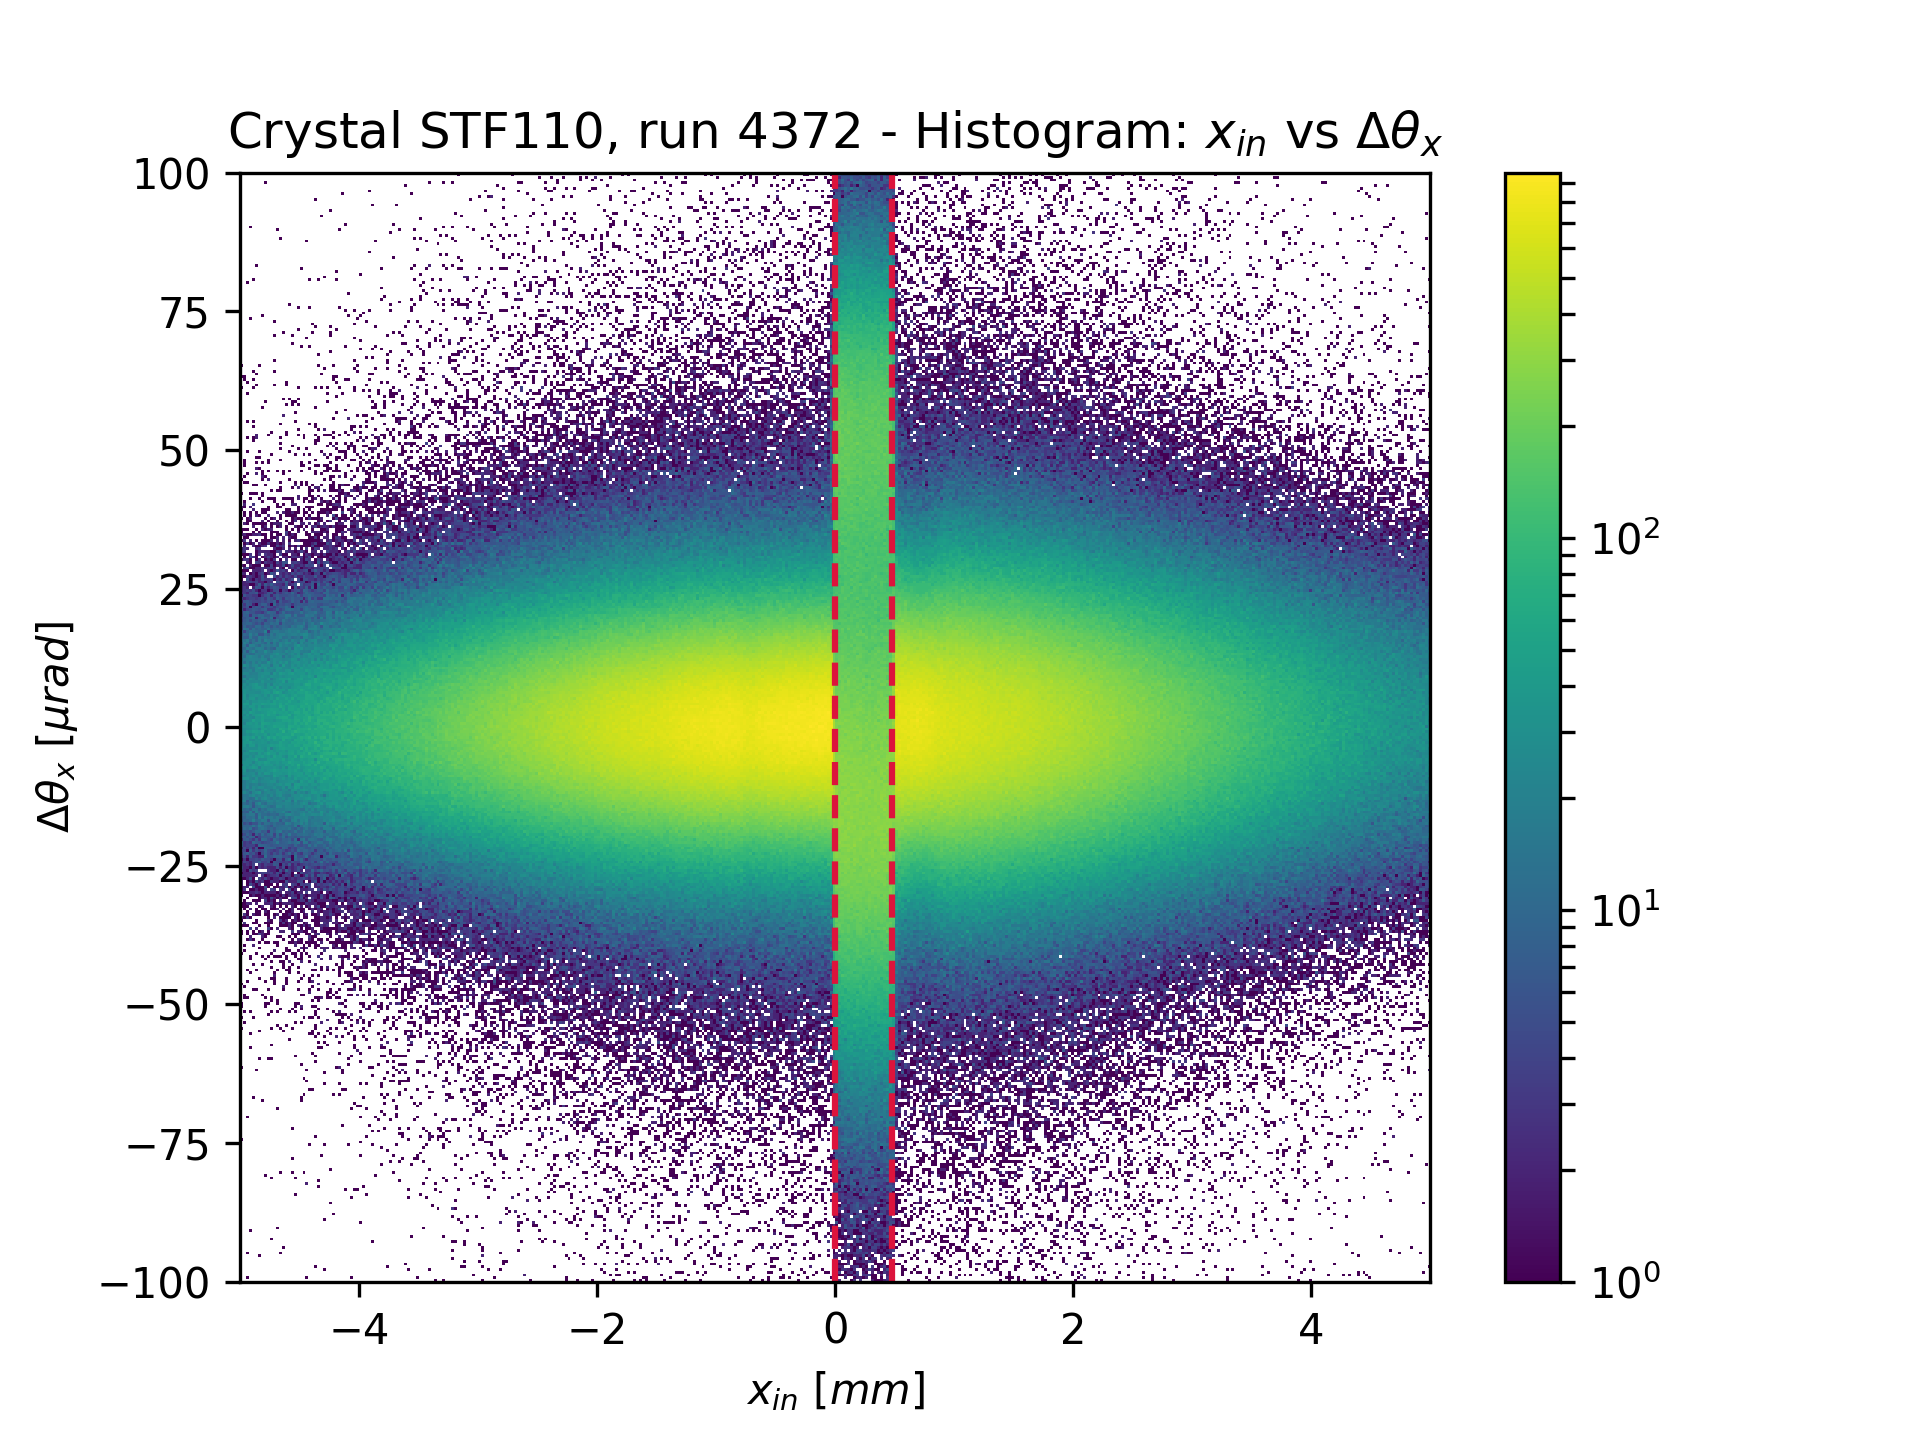
\includegraphics[width=0.8\linewidth]{test}
% %\end{figure}
% \end{frame}
% 
% %------------------------------------------------
% 
% \begin{frame}[fragile] % Need to use the fragile option when verbatim is used in the slide
% \frametitle{Citation}
% An example of the \verb|\cite| command to cite within the presentation:\\~
% 
% This statement requires citation \cite{p1}.
% \end{frame}
% 
% %------------------------------------------------
% 
% \begin{frame}
% \frametitle{References}
% \footnotesize{
% \begin{thebibliography}{99} % Beamer does not support BibTeX so references must be inserted manually as below
% \bibitem[Smith, 2012]{p1} John Smith (2012)
% \newblock Title of the publication
% \newblock \emph{Journal Name} 12(3), 45 -- 678.
% \end{thebibliography}
% }
% \end{frame}
% 
% %------------------------------------------------
% 
% \begin{frame}
% \Huge{\centerline{The End}}
% \end{frame}
% 
% %----------------------------------------------------------------------------------------

\end{document} 